
%%%%%%%%%%%%%%%%%%%%%%%%%%%%%%%%%%%%%%%%%%%%%%%%
% 1. Document Class
%%%%%%%%%%%%%%%%%%%%%%%%%%%%%%%%%%%%%%%%%%%%%%%%
 
 % The first command you will always have will declare your document class. This tells LaTeX what type of document you are creating (article, presentation, poster, etc). 
% \documentclass is the command
% in {} you specify the type of document
% in [] you define additional parameters
 
\documentclass[a4paper,12pt]{article} % This defines the style of your paper

% We usually use the article type. The additional parameters are the format of the paper you want to print it on and the standard font size. For us this is a4paper and 12pt.

%%%%%%%%%%%%%%%%%%%%%%%%%%%%%%%%%%%%%%%%%%%%%%%%
% 2. Packages
%%%%%%%%%%%%%%%%%%%%%%%%%%%%%%%%%%%%%%%%%%%%%%%%

% Packages are libraries of commands that LaTeX can call when compiling the document. With the specialized commands you can customize the formatting of your document.
% If the packages we call are not installed yet, TeXworks will ask you to install the necessary packages while compiling.

% First, we usually want to set the margins of our document. For this we use the package geometry. We call the package with the \usepackage command. The package goes in the {}, the parameters again go into the [].
\usepackage[top = 2.5cm, bottom = 2.5cm, left = 2.5cm, right = 2.5cm]{geometry} 

% Unfortunately, LaTeX has a hard time interpreting German Umlaute. The following two lines and packages should help. If it doesn't work for you please let me know.
\usepackage[T1]{fontenc}
\usepackage[utf8]{inputenc}

% The following two packages - multirow and booktabs - are needed to create nice looking tables.
\usepackage{multirow} % Multirow is for tables with multiple rows within one cell.
\usepackage{booktabs} % For even nicer tables.

% As we usually want to include some plots (.pdf files) we need a package for that.
\usepackage{graphicx} 

% The default setting of LaTeX is to indent new paragraphs. This is useful for articles. But not really nice for homework problem sets. The following command sets the indent to 0.
\usepackage{setspace}
\setlength{\parindent}{0in}

% Package to place figures where you want them.
\usepackage{float}

% The fancyhdr package let's us create nice headers.
\usepackage{fancyhdr}


%%%%%%%%%%%%%%%%%%%%%%%%%%%%%%%%%%%%%%%%%%%%%%%%
% 3. Header (and Footer)
%%%%%%%%%%%%%%%%%%%%%%%%%%%%%%%%%%%%%%%%%%%%%%%%

% To make our document nice we want a header and number the pages in the footer.

\pagestyle{fancy} % With this command we can customize the header style.

\fancyhf{} % This makes sure we do not have other information in our header or footer.

\lhead{\footnotesize GEO1001: Assignment 1}% \lhead puts text in the top left corner. \footnotesize sets our font to a smaller size.

%\rhead works just like \lhead (you can also use \chead)
\rhead{\footnotesize Theodoros Papakostas (5287928)} %<---- Fill in your lastnames.

% Similar commands work for the footer (\lfoot, \cfoot and \rfoot).
% We want to put our page number in the center.
\cfoot{\footnotesize \thepage} 


%%%%%%%%%%%%%%%%%%%%%%%%%%%%%%%%%%%%%%%%%%%%%%%%
% 4. Your document
%%%%%%%%%%%%%%%%%%%%%%%%%%%%%%%%%%%%%%%%%%%%%%%%

% Now, you need to tell LaTeX where your document starts. We do this with the \begin{document} command.
% Like brackets every \begin{} command needs a corresponding \end{} command. We come back to this later.
\usepackage{float}
\begin{document}


%%%%%%%%%%%%%%%%%%%%%%%%%%%%%%%%%%%%%%%%%%%%%%%%
%%%%%%%%%%%%%%%%%%%%%%%%%%%%%%%%%%%%%%%%%%%%%%%%

%%%%%%%%%%%%%%%%%%%%%%%%%%%%%%%%%%%%%%%%%%%%%%%%
% Title section of the document
%%%%%%%%%%%%%%%%%%%%%%%%%%%%%%%%%%%%%%%%%%%%%%%%

% For the title section we want to reproduce the title section of the Problem Set and add your names.

\thispagestyle{empty} % This command disables the header on the first page. 

\begin{tabular}{p{15.5cm}} % This is a simple tabular environment to align your text nicely 
{\large \bf Sensing Technologies and Mathematics for Geomatics} \\
GEO1001.2020 \\ MSc Geomatics \\ Delft University of Technology \\
\hline % \hline produces horizontal lines.
\\
\end{tabular} % Our tabular environment ends here.

\vspace*{2.8cm} % Now we want to add some vertical space in between the line and our title. 
\begin{center}
	 % Everything within the center environment is centered.
	{\Large \bf\  Assignment 1} % <---- Don't forget to put in the right number
	\vspace{5mm}
	
        % YOUR NAMES GO HERE
	{\bf\ Theodoros Papakostas (5287928)} % <---- Fill in your names here!
\end{center}  
\vspace{1cm}
%%%%%%%%%%%%%%%%%%%%%%%%%%%%%%%%%%%%%%%%%%%%%%%%
%%%%%%%%%%%%%%%%%%%%%%%%%%%%%%%%%%%%%%%%%%%%%%%%
{Introduction:}
For this assignment we use data collected from 5 heat stress sensors placed somewhere in the Netherlands during this summer. The sensors are Kestrel 5400 and their specs are included within the assignment materials. In order to identify if the dataset is of any value to our “employer”, it is our job to deeply analyse the dataset and derive hypothesis from it.\cite{Maiullari2020}
\pagebreak 
\section{Lecture A1}
\vspace{10mm}
\subsection{Mean Statistics}
\vspace{5mm}
\setlength{\parindent}{8ex}First of all, given the datasets of 5 sensors(A,B,C,D,E) with measurements over 19 variables, mean statistics (mean, variance and standard deviation) were computed.\cite{Maiullari2020}The results are aggregated  on the matrices underneath this subsection.

\setlength{\parindent}{8ex} In general, the mean statistics(mean,variance,standard deviation), fluctuate in ordinary values and no peculiar behaviors over them can be identified. Thus, we cannot yet reach any statistically significant conclusions over them, nor derive any robust hypothesis from them. Especially when, we have to do with 19 different variables, leads to the need of more circumstantial analysis. 
\vspace{10mm}
 \begin{figure}[H]   
	\centering 
	\includegraphics[width=0.9\textwidth]{Mean_Statistics.png}
	\caption{Mean statistics of the 5 sensors} 
\end{figure}
\vspace{10mm}
\subsection{Histograms for the 5 sensors values}
\vspace{5mm}
Given the Temperature values of the 5 sensors, 2 histograms were created: 1 using 5 bins and 1 using 50 bins.

\setlength{\parindent}{8ex}Those histograms graphically display the shape of the distribution, for each sensor's measurement values.This is really useful in particular, because we have to deal with a big load of observations. However, in order to take  full advantage of this specific visualisation, the choice of bin number to be used is very important. Rice's formula on the choice of bin number, is generally used : \[2\times\sqrt[3]{N}\]

\setlength{\parindent}{8ex}In our case, the two different bin choices we made, result in two apparently different histograms. On the on side, as we observe on Figure 2, the 5-bin selection leads to a very generic visualisation of the distribution which apparently disregards any peculiar data fluctuation impacts. Thus, even though we have acquired a large number of observations we cannot make full use of it to identify discrete unordinary data behavior,of the 5 sensors. On the other side, as we observe on Figure 3, the 50-bin selection demonstrates a very detailed distribution of the 5 sensors' measurements out of which, useful information can be extracted.However, this accumulated detail, may lead to difficulties in discriminating the correct information. Consequently, the choice of the number of bins to be used is very important.
\vspace{10mm}
 \begin{figure}[H]   
	\centering 
	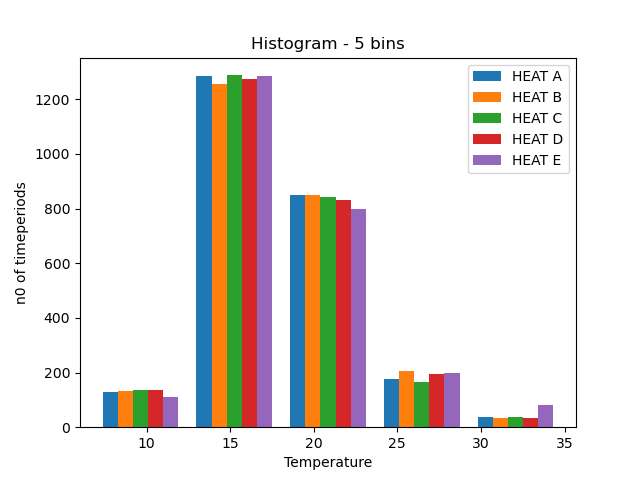
\includegraphics[width=0.7\textwidth]{Figure_1.png}
	\caption{Histogram -5 sensors Temperature} 
\end{figure}
 \begin{figure}[H]   
	\centering 
	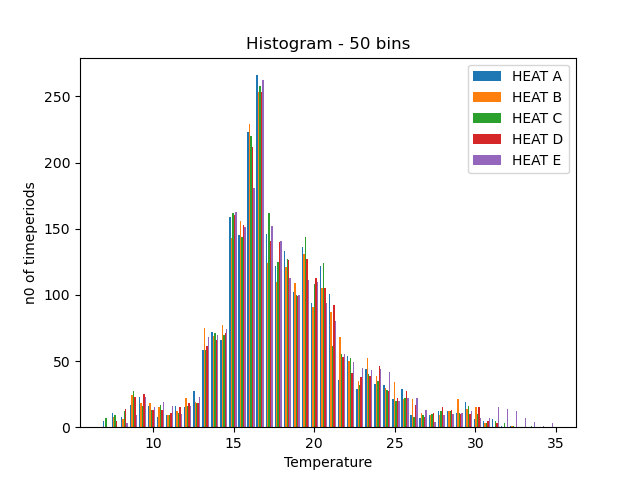
\includegraphics[width=0.7\textwidth]{Figure_2.png}
	\caption{Histogram -5 sensors Temperature} 
\end{figure}
	
\subsection{Frequency polygons for the 5 sensors' Temperature}
\vspace{5mm}
On this subsection, a plot was created, where frequency polygons for the 5 sensors Temperature overlap in different colors. The No of bins is 27. Choice was made using the Rice's formula for N=2476.
 \begin{figure}[H]   
	\centering 
	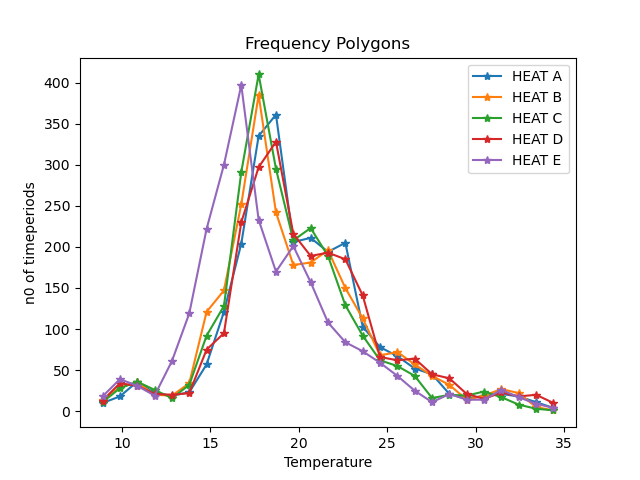
\includegraphics[width=0.7\textwidth]{Figure_3.png}
	\caption{Frequency polygons} 
\end{figure}
\vspace{10mm}
\subsection{5 sensors boxplots for: Wind Speed, Wind Direction, Temperature}
\vspace{5mm}
Over here, 3 particular boxplots were generated, containing information for the 5 sensors Wind Speed, Wind Direction and Temperature. The boxplots,in general, are used to identify any outliers and for comparing distributions.

\setlength{\parindent}{8ex}In particular, on the created boxplots, we can observe that for those 3 variables, the 4 sensors behave almost similarly. On the contrary, the E sensor features some dissimilarities concerning its outliers. This is really aparrent, especially in the boxplot for the Wind Direction.
 \begin{figure}[H]   
	\centering 
	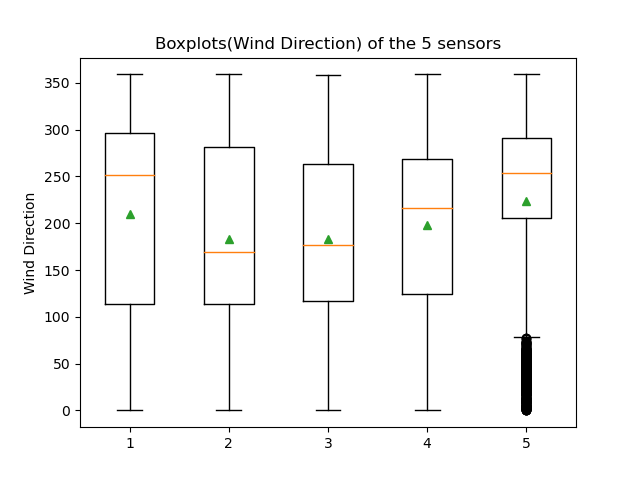
\includegraphics[width=0.5\textwidth]{Figure_4.png}
	\caption{Plot 1} 
\end{figure}
 \begin{figure}[H]   
	\centering 
	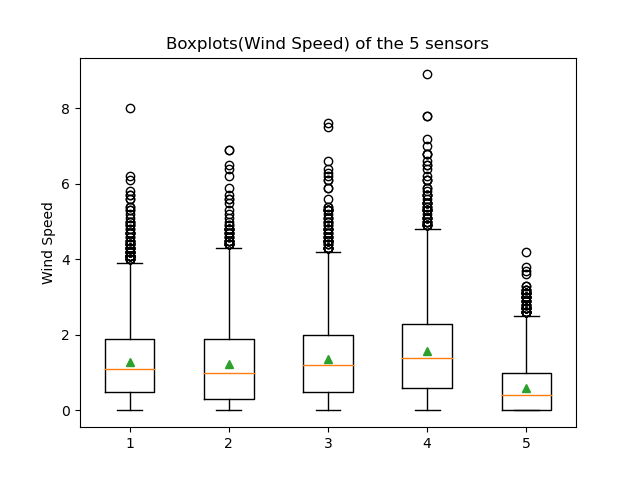
\includegraphics[width=0.5\textwidth]{Figure_5.png}
	\caption{Plot 2} 
\end{figure}
 \begin{figure}[H]   
	\centering 
	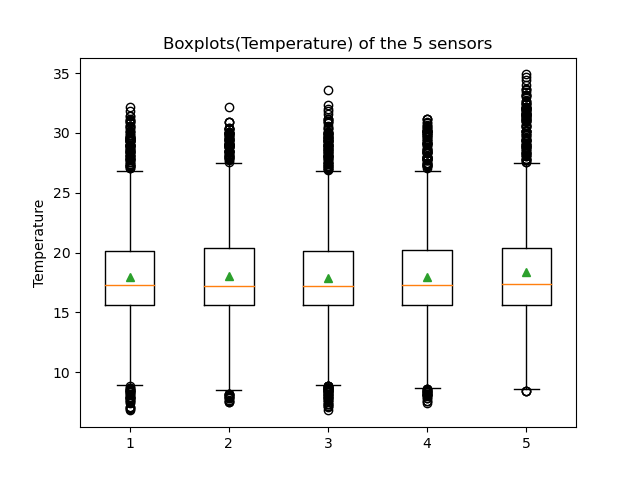
\includegraphics[width=0.5\textwidth]{Figure_6.png}
	\caption{Plot 3} 
\end{figure}
\section{Lecture A2}
\vspace{10mm}
\subsection{PMF, PDF, CDF for the 5 sensors' Temperature}
\vspace{5mm}
Using the 5 sensors' Temperature variable, the PMF,PDF,CDF of each one was plot.
\vspace{10mm}
\begin{figure}[H]   
	\centering 
	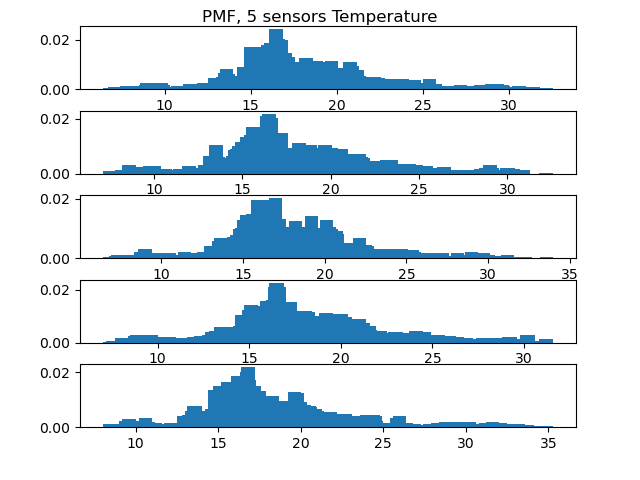
\includegraphics[width=0.9\textwidth]{Figure_7.png}
	\caption{Probability Mass Function, 5 sensors} 
\end{figure}
\vspace{5mm}
\setlength{\parindent}{8ex} Probability Mass Functions(PMFs), is a way to represent a distribution of each value's probability. It is a bar chart where we get from frequency to probability, through the division by N(number of values), in order to succeed normalization. A way not to be mislead by the different sample sizes. Indeed, the temperature variable values were not the same for every sensor. In general terms, the PMFs for the 5 sensors, have the same behavior concerning their main bodies. As for their tails, we observe that the probability rates decline proportionally to the maximum and minimum temperature values.
\vspace{10mm}
\begin{figure}[H]   
	\centering 
	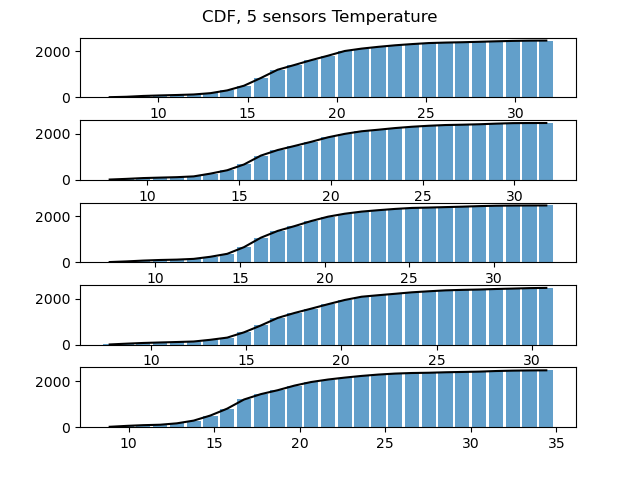
\includegraphics[width=0.7\textwidth]{Figure_9.png}
	\caption{Cumulative Density Function, 5 sensors} 
\end{figure}
\begin{figure}[H]   
	\centering 
	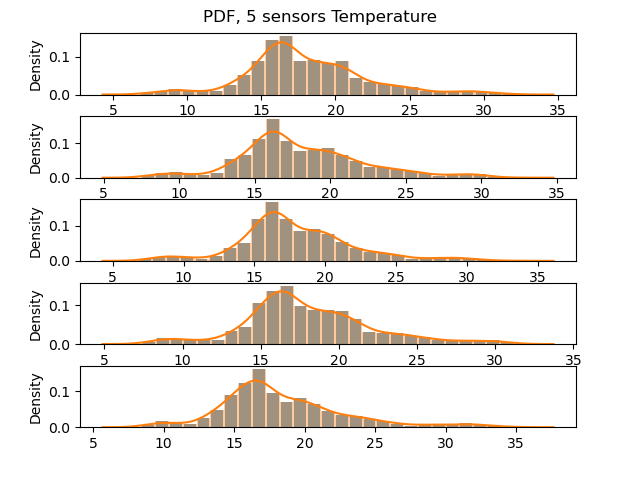
\includegraphics[width=0.7\textwidth]{Figure_8.png}
	\caption{Probability Density Function, 5 sensors} 
\end{figure}
\vspace{5mm}
\setlength{\parindent}{8ex}The Cumulative Density Function(CDF) map from a value to its percentile rank. Its derivative is called Probability Density Function(PDF) and actually measures the probability pes unit of x. 

\setlength{\parindent}{8ex}The behavior of both distributions CDF and PDF, looks similar in general, for the 5 sensors, and there is not any significant disimilarity to be noted.
\subsection{PDF and Kernel density estimation, 5 sensors Wind Speed values}
\vspace{10mm}
For the Wind Speed values, the PDF and Kernel Density Estimation were plotted.
\vspace{15mm}
\begin{figure}[H]   
	\centering 
	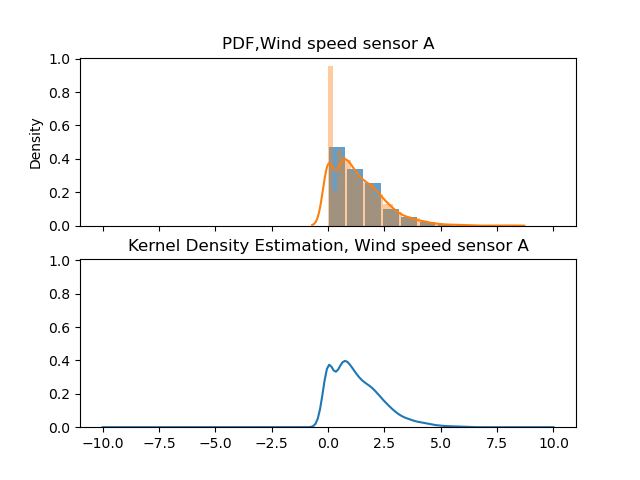
\includegraphics[width=0.5\textwidth]{Figure_10.png}
	\caption{sensor A - Wind speed} 
\end{figure}
\begin{figure}[H]   
	\centering 
	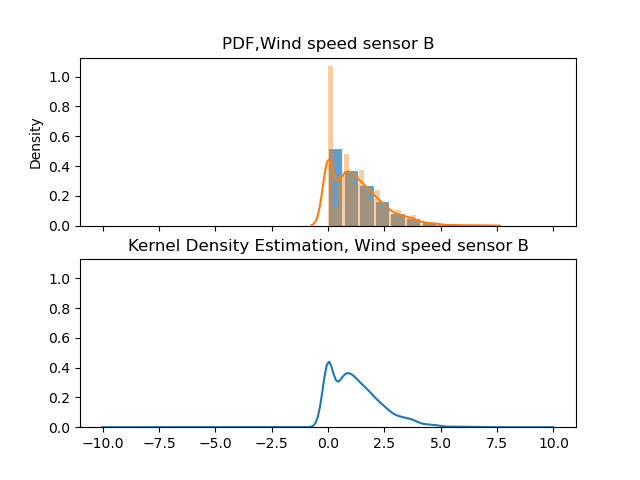
\includegraphics[width=0.5\textwidth]{Figure_11.png}
	\caption{sensor B - Wind speed} 
\end{figure}
\begin{figure}[H]   
	\centering 
	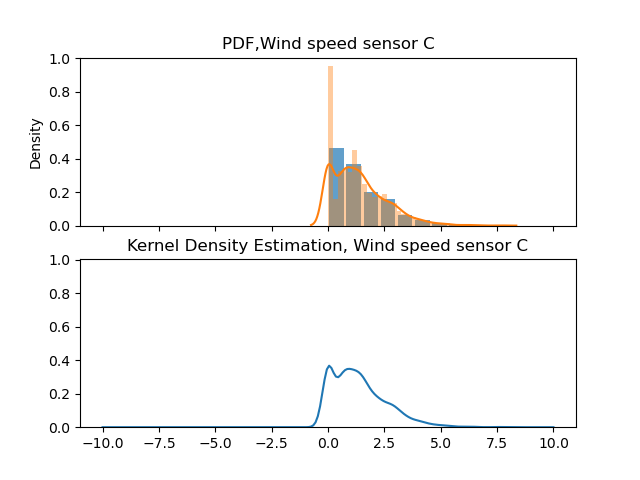
\includegraphics[width=0.5\textwidth]{Figure_12.png}
	\caption{sensor C - Wind speed} 
\end{figure}
\begin{figure}[H]   
	\centering 
	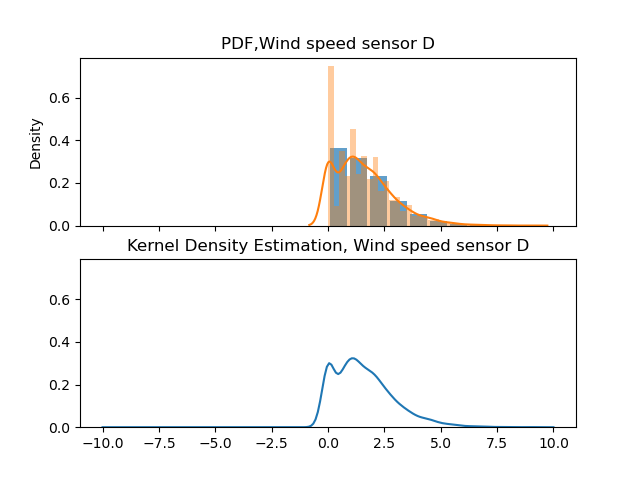
\includegraphics[width=0.5\textwidth]{Figure_13.png}
	\caption{sensor D - Wind speed} 
\end{figure}
\begin{figure}[H]   
	\centering 
	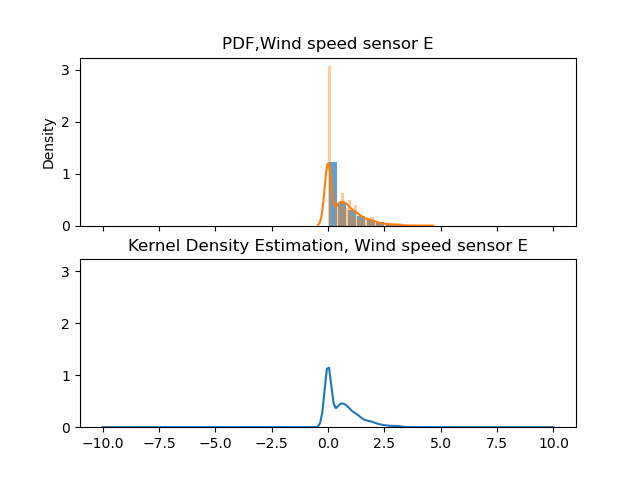
\includegraphics[width=0.5\textwidth]{Figure_14.png}
	\caption{sensor E - Wind speed} 
\end{figure}

\setlength{\parindent}{8ex} We can observe that for all the 5 sensors, the PDF and the KDE are almost identical. Of course, this comes as no surprise, since the KDE is actually an algorithm takes a sample and constructs an appropriately smooth PDF that fits those data. Thus, that's what happens in this incident, with the Wind values of each sensor.
\section{Lecture A3}
\subsection{Coorelation and Coefficients}
Correlations were computed between all the sensors for the variables: Temperature, Wet Bulb Globe Temperature (WBGT), Crosswind Speed. For this purpose, Pearson’s and Spearmann’s rank coefficients were used. At last, a scatter plot with both coefficients with the 3 variables was plot.
\begin{figure}[H]   
	\centering 
	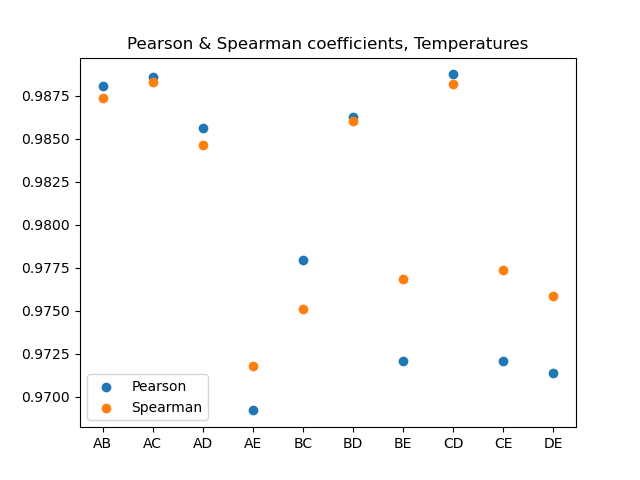
\includegraphics[width=0.4\textwidth]{Figure_15.png}
	\caption{Coorelation - Temperature} 
\end{figure}
\begin{figure}[H]   
	\centering 
	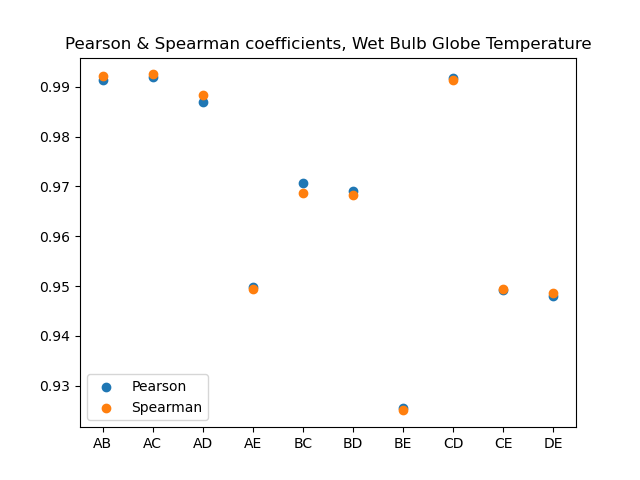
\includegraphics[width=0.4\textwidth]{Figure_16.png}
	\caption{Coorelation -  Wet Bulb Globe Temperature} 
\end{figure}
\begin{figure}[H]   
	\centering 
	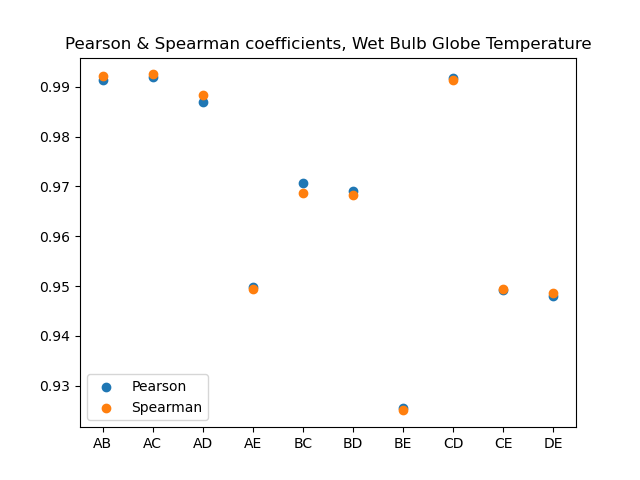
\includegraphics[width=0.4\textwidth]{Figure_16.png}
	\caption{Coorelation -  Crosswind Speed} 
\end{figure}
\vspace{7mm}
\subsection{Coorelations}
\setlength{\parindent}{8ex}Something that can easily be spot, on the scatter plots of the coefficients, is that both Temperature and WBGTemperature have high coorelation(values are over 0.97), for all the sensors. This is logical because they both have to do with temperature values which is less likely to have great ups and downs in a particular place. Addittionally, those variables' values of all the sensors have a linear relationship that could be seen from the values scatter plot, which also shows their great coorelation. On the contrary, Crosswind speed has a lot smaller coorelation values between the sensors(from 0.4 to 0.65), due to its non-linear relationship that could be seen from the values scatter plots. Generally we note great coorelation between the sensors' values for Temperature,Wet Bulb Globe Temperature, and a lot less coorelation between the sensors' values for Crosswind speed.
\subsection{Hypothesis}
\setlength{\parindent}{8ex}As mentioned before, if we observe the scatter plots of the values for the variables Temperature, Wet Bulb Globe Temperature and Crosswind Speed we reach the conclusion that for the 5 sensors the relationships between Temperatures are linear and between Crosswind Speeds are not linear. We take advantage of the Spearman rank coefficients that are more robust for non linear relationships, and thus, we note that in the Crosswind Speed coefficients scatter plot the sensors C and D have the greatest coorelation. In parallel, this high coorelation between C and D is also visible in the other two coefficient scatter plots(temperature). That's why I assume that  C and D must be really close, and may be the two neighbour sensors on the left side. Now, I observe that C and D are less coorelated on the Crosswind scatter, with E sensor, which I assume that is the one top right. Also, on the Temperature scatter plots, we can observe that AC,AD have high coorelation values,higher that BC,BD so we can assume the exact position of A and B(B up, A down, because it is closer to C and D ).So, at last, we can conclude to the final hypothesis for the sensors' locations.
\vspace{5mm}
\begin{figure}[H]   
	\centering 
	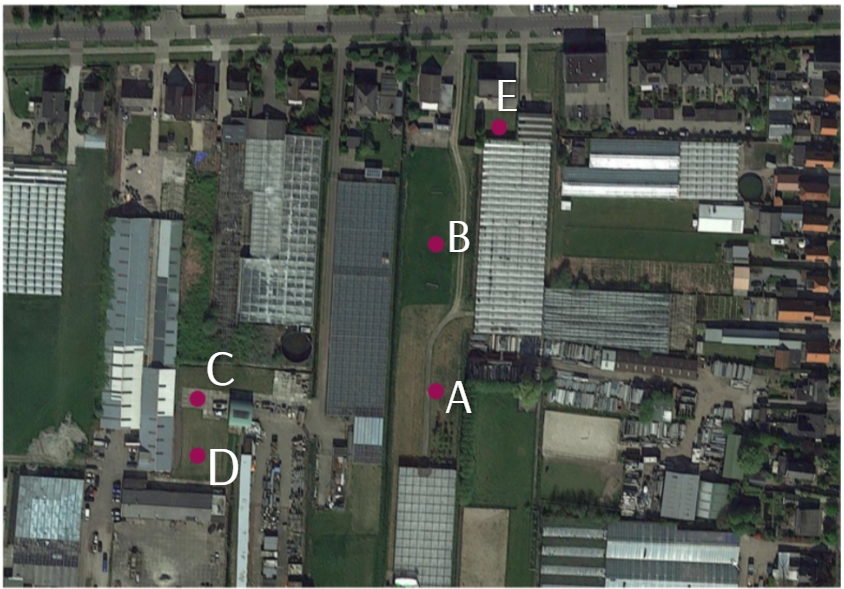
\includegraphics[width=0.7\textwidth]{Hypothesis.png}
	\caption{Hypothetical sensors locations} 
\end{figure}
\section{Lecture A4}
\vspace{5mm}
\subsection{CDF for 5 sensors' Temperature and Wind Speed, 95 percent confidence intervals}
\vspace{10mm}
 In this part, the CDF for all the sensors and for variables Temperature and Wind Speed, were plot. Then the 95 percent confidence intervals for variables Temperature and Wind Speed for all the sensors were computed and saved in a table (csv form). The table can be seen underneath.
 \vspace{10mm}
\begin{figure}[H]   
	\centering 
	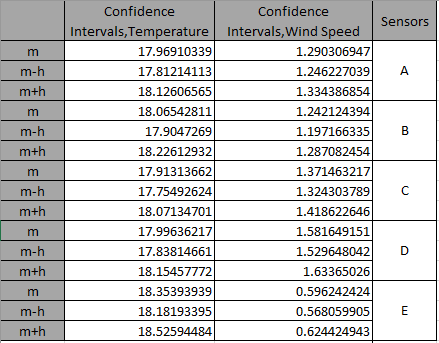
\includegraphics[width=0.4\textwidth]{Confidence_intervals.png}
	\caption{95 percent Cofidence Intervals } 
\end{figure}
\begin{figure}[H]   
	\centering 
	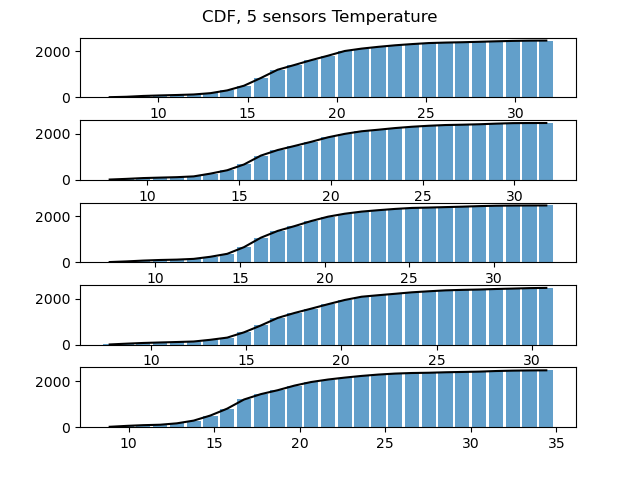
\includegraphics[width=0.5\textwidth]{Figure_9.png}
	\caption{CDF, 5 sensors } 
\end{figure}
\begin{figure}[H]   
	\centering 
	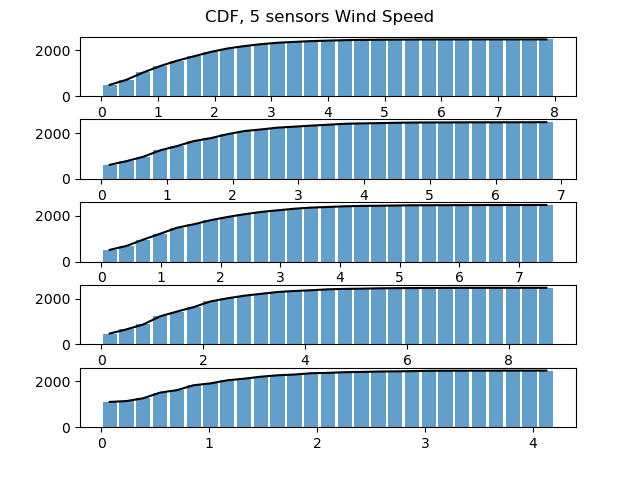
\includegraphics[width=0.5\textwidth]{Figure_18.png}
	\caption{CDF, 5 sensors } 
\end{figure}
\subsection{Hypothesis test}
\vspace{5mm}
Test the hypothesis: the time series for Temperature and Wind Speed are the same for sensors:

1) E, D;

2) D, C;

3) C, B;

4) B, A;
\vspace{10mm}

\setlength{\parindent}{8ex}T.test:The null hypothesis over those four cases,returns the t and the p value for each variable(Temperature,Wind Speed).The p value shows which is the probability of seeing the apparent effect if the
null hypothesis is true. A p-value higher than 0.05(p>0.05), is not statistically significant and indicates strong evidence for the null hypothesis. If the p-value is near 0, the effect is said to be statistically significant, which means it is unlikely to have occured by chance. The t.test results are shown in the table underneath.
\vspace{5mm}
\begin{figure}[H]   
	\centering 
	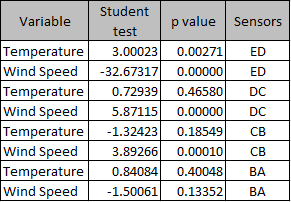
\includegraphics[width=0.6\textwidth]{T_test.png}
	\caption{T.test results} 
\end{figure}
\section{Bonus Question}
\vspace{10mm}
My “employer” wants to estimate the day of maximum and minimum potential energy consumption due to air conditioning usage. To hypothesize regarding those days, I am asked to identify the hottest and coolest day of the measurement time series provided.

\setlength{\parindent}{8ex}To do that, in the beginning, I defined a function that fills a dictionary like this: first column with the mean temperatures of every day data set given, and second column with the days count. The measurement frequency is 20 minutes. Thus, I calculate the mean for every 72 cells of measurements dataset, and I get a final dictionary with 34 mean temperatures, and 34 days,placed proportionally. I name the dictionary to a Dataframe so I can sort it. I sort the dataframe, by the values of the mean temperatures. Thus, in the end I get a sorted dataframe that starts from the hottest to the coolest mean temperature, and the days those mean temperatures took place. I call this function 5 times, for each sensor, and I print the results for the hottest and coolest days. The results are :
\begin{figure}[H]   
	\centering 
	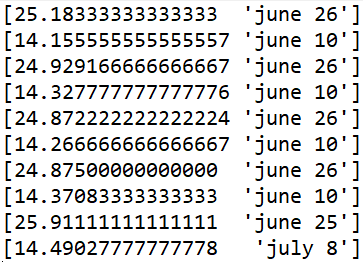
\includegraphics[width=0.4\textwidth]{MaxMin.png}
	\caption{Max-min temperatures} 
\end{figure}
\vspace{5mm}

\setlength{\parindent}{8ex} As we observe, the 4 sensors have identical results(june 26',june '10). The sensor E indicates an other result(june '25,july '8), however, there is a really slight difference if we check the sorted dataframe, with the upper results(june 26',june '10). Consequently, I conclude :

\setlength{\parindent}{12ex}hottest day: June 26th

\setlength{\parindent}{12ex}coolest day: June 10th


\bibliographystyle{plain}

\bibliography{bibliography}

\end{document}